\documentclass[a4paper]{article}

%% Language and font encodings
\usepackage[english]{babel}
\usepackage[utf8x]{inputenc}
\usepackage[T1]{fontenc}

%% Sets page size and margins
\usepackage[a4paper,top=3cm,bottom=2cm,left=3cm,right=3cm,marginparwidth=1.75cm]{geometry}

%% Useful packages
\usepackage{amsmath}
\usepackage{graphicx}
\usepackage{caption}
\usepackage{subcaption}
\usepackage[colorinlistoftodos]{todonotes}
\usepackage[colorlinks=true, allcolors=blue]{hyperref}

\title{Reporte de Actividad 6: Sistema de Resortes Acoplados}
\author{Jesús Antonio González Espinosa \\ \\ Física Computacional 1}
\date{Martes, 20 de Marzo del 2018}

\begin{document}
\maketitle

\section{Introducción}

Para esta actividad hemos trabajado con modelación de fenómenos físicos en python; específicamente en el de oscilaciones, presentando varios ejemplos de sistemas de resortes acoplados.

En este reporte se presenta la síntesis de los primeros dos subtemas del documento "Coupled spring equations" de TEMPLE H. FAY, el cual nos aporta la teoría necesaria para obtener las bases y comprender los conceptos importantes para poder efectuar la actividad. Asimismo, el documento dio las propiedades y condiciones iniciales de las gráficas presentadas en este reporte. Naturalmente, se presenta el cierre al reporte, incluyendo bilbiografía, conclusiones y el apéndice perteneciente a la actividad.

\section{Sintesis}
\subsection{Introducción}
En éste artículo se investiga el problema de los dos resortes y dos pesas adjuntas en serie. Bajo la suposición de que las fuerzas de restauración se comportan de acuerdo a la Ley de Hooke, este problema de dos grados de libertad es modelado por un par de ecuaciones diferenciales lineales de segundo orden que al sustituir una en la otra, el movimiento de cada pesa puede ser determinado por una ecuación diferencial lineal de cuarto orden. 

Lo que hace interesante a este problema, es que podemos investigar los movimientos de las masas, para ver si están sincronizadas u opuestas entre ellas. También se puede ver que al agregarle factores no lineares, pueden surgir movimientos interesantes. Al modificar los parámetros podemos observar gráficamente los cambios en la periodicidad, la amplitud, la fase, la sensitividad a loas condiciones iniciales, entre otras propiedades. 

\subsection{El modelo de resorte acoplado}
El modelo consiste en dos resortes y dos pesas. Un resorte tiene la constante elástica $k_1$ y está adjunto al techo de un extremo y del otro tiene una pesa de masa $m_1$. La misma pesa tiene adjunto un segundo resorte de constante elástica $k_2$ y al final de éste, una pesa de masa $m_2$. Al dejar el sistema llegar al equilibrio, medimos el desplazamiento de cada masa, en función del tiempo, y llamaremos estas medidas como: $x_1(t)$ y $x_2(t)$.

\begin{figure}[h]
 \centering
  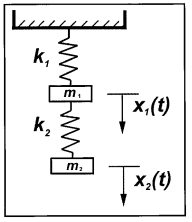
\includegraphics[width=0.2\textwidth]{ModeloResorte.PNG}
\end{figure}

\subsubsection{Asumiendo la Ley de Hooke}
Asumiendo que hay pequeñas oscilaciones, las fuerzas restauradoras son de la forma $- k_1l_1$ y $- k_2l_2$, donde $l_1$ y $l_2$ son las elongaciones o compresiones de los dos resortes. Como la masa superior está unida a ambos resortes, ésta siente las dos fuerzas restauradoras actuando sobre ella, mientras que la segunda masa solo siente la fuerza restauradora del segundo resorte. Asumiendo que no hay fuerzas de amortiguamiento, la Ley de Newton implica que las ecuaciones que representan los movimientos de las pesas son:

\begin{center}
$m_1\ddot x_1 = - k_1x_1 - k_2(x_1 - x_2)$

$m_1\ddot x_2 = - k_2(x_1 - x_2)$
\end{center}

Entonces para encontrar una ecuación para $x_1$ que no involucre a $x_2$, resolvemos la primera ecuación diferencial para $x_2$, y la sustituimos en la primera, donde después de simplificar, obtenemos:

\begin{center}
$m_1m_2x_1^{(4)} + (m_2k_1 + k_2(m_1 + m_2))\ddot x_1 + k_1k_2x_1 = 0$
\end{center}

Ahora, para encontrar una ecuación que involucre de $x_2$, resolvemos la segunda ecuación diferencial para $x_1$ y lo sustituimos en la primera ecuación, obteniendo:

\begin{center}
$m_1m_2x_2^{(4)} + (m_2k_1 + k_2(m_1 + m_2))\ddot x_1 + k_1k_2x_2 = 0$
\end{center}

Para poder resolver las ecuaciones, solo es necesario las posiciones iniciales y las velocidades iniciales.

\subsubsection{Algunos ejemplos con masas idénticas}
Consideremos el modelo con dos pesas con la misma masa, $m_1 = m_2 = 1$, ignorando el amortiguamiento y sin fuerzas externas.

\textbf{Ejemplo 2.1:} Describe el movimiento para las constantes de resorte $k_1 = 6$ y $k_2 = 4$ con las condiciones iniciales ($x_1(0), \dot x_1(0), x_2(0), \dot x_2(0)) = (1,0,2,0)$.
Al resolverlo de manera analítica obtenemos:
\begin{center}
$x_1(t) = cos \sqrt{2}t$

$x_2(t) = 2 cos \sqrt{2}t$
\end{center}

El movimiento es sincronizado, por lo tanto, las pesas se mueven en fase una con la otra, teniendo el mismo periodo, pero con amplitudes un poco diferentes. 

Para poder grafciar esto en Python, utilizamos un código proporcionado. Este código se utilizó durante toda la actividad, solo modificando los parámetros y condiciones iniciales; así como las variables de los ejes coordenados para presentar las diferentes gráficas. En este caso, el código para este ejemplo se ve así:

\begin{figure}[ht!]
 \centering
  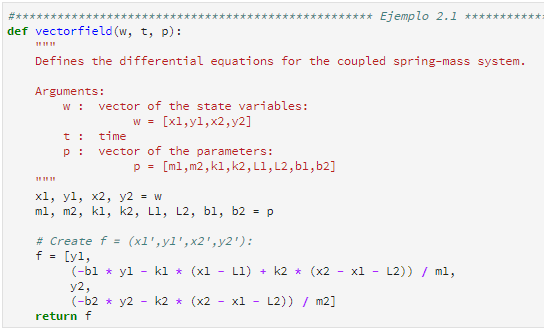
\includegraphics[width=0.65\textwidth]{Codigo1.PNG}
\end{figure}
\pagebreak
\begin{figure}[ht!]
 \centering
  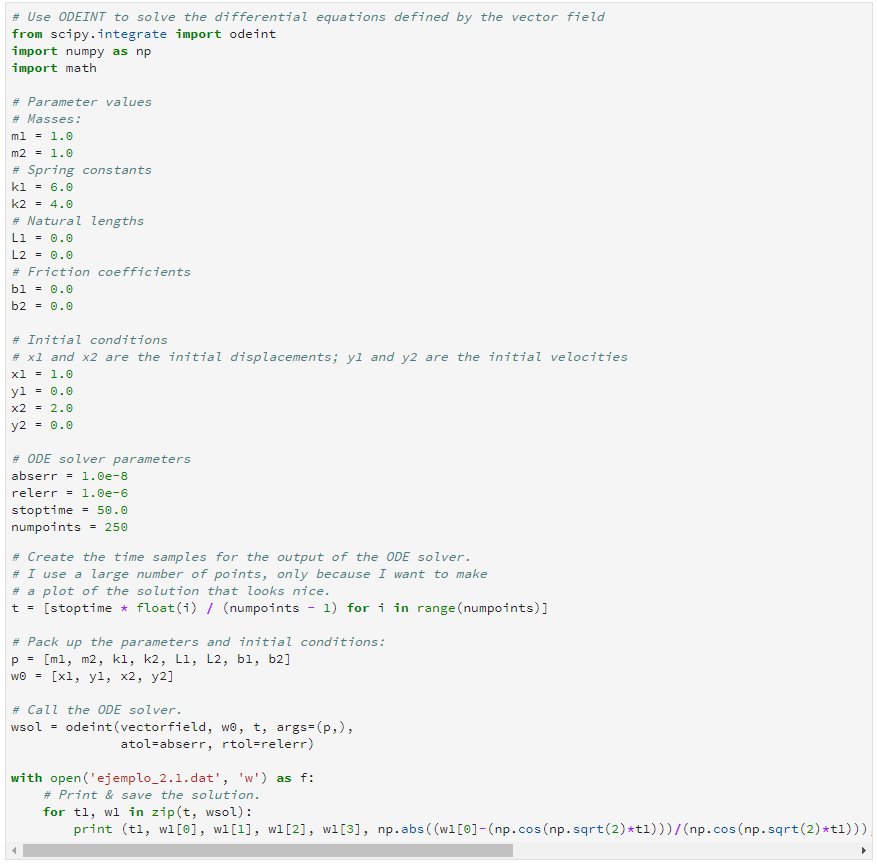
\includegraphics[width=0.65\textwidth]{Codigo2.PNG}
\end{figure}
\begin{figure}[ht!]
 \centering
  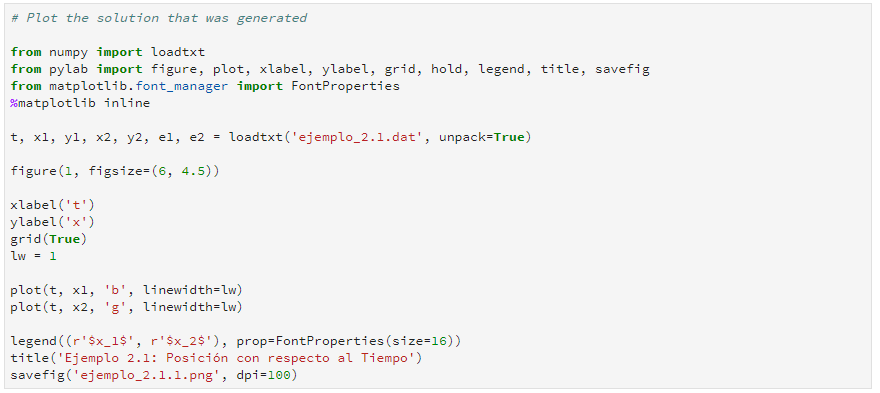
\includegraphics[width=0.65\textwidth]{Codigo3.PNG}
\end{figure}
Obteniendo las siguientes gráficas:
\begin{figure}[h!]
 \centering
  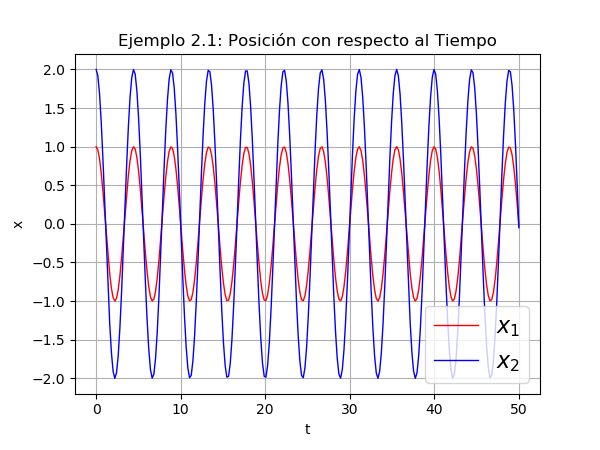
\includegraphics[width=0.65\textwidth]{ejemplo_2_1_1.png}
  \caption{Posición con respecto al Tiempo de $x_1$ y $x_2$}
\end{figure}

\pagebreak
\begin{figure}[ht!]
\begin{subfigure}{0.6\textwidth}
  \centering
  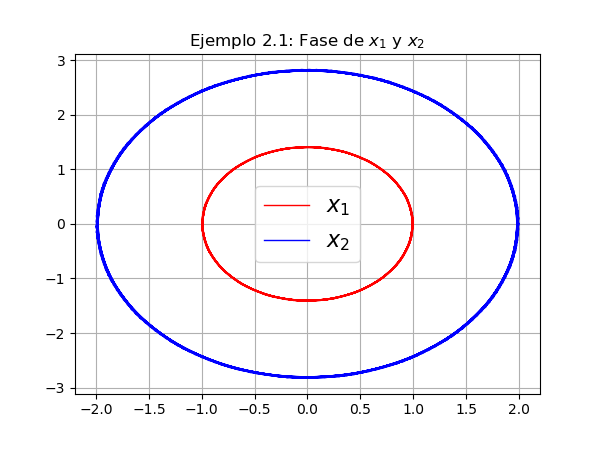
\includegraphics[width=\linewidth]{ejemplo_2_1_3.png}
   \caption{Fase de $x_1$ y $x_2$}
\end{subfigure}
\begin{subfigure}{0.6\textwidth}
  \centering
  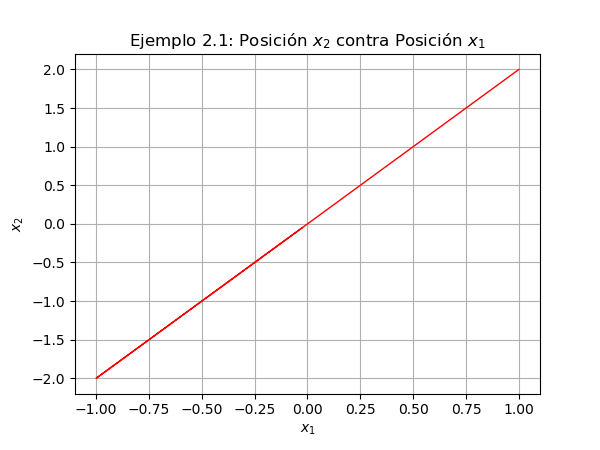
\includegraphics[width=\linewidth]{ejemplo_2_1_2.png}
  \caption{Posición $X_2$ contra $x_1$}
\end{subfigure}
\end{figure}

El error relativo de $x_1$ y $x_2$:

\begin{figure}[ht!]
\begin{subfigure}{0.6\textwidth}
  \centering
  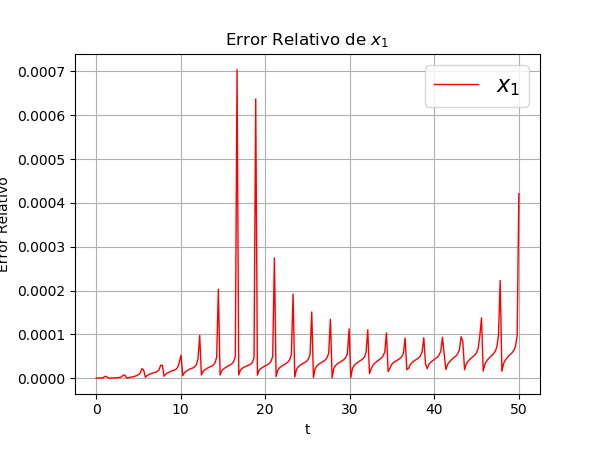
\includegraphics[width=\linewidth]{error2_1_1.png}
   \caption{Error Relativo de $x_1$}
\end{subfigure}
\begin{subfigure}{0.6\textwidth}
  \centering
  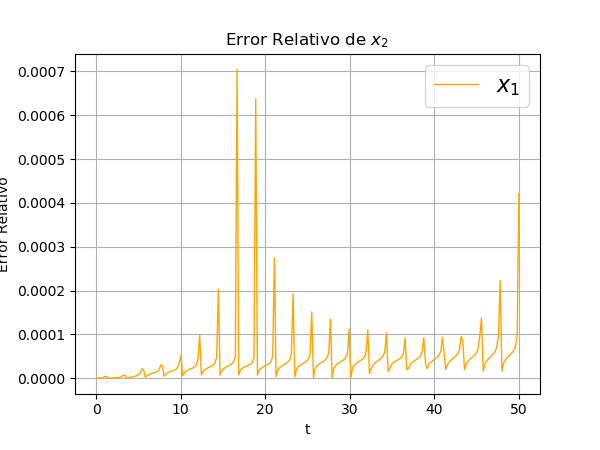
\includegraphics[width=\linewidth]{error2_1_2.png}
  \caption{Error Relativo de $x_2$}
\end{subfigure}
\end{figure}

\bigskip

\textbf{Ejemplo 2.2:} Describe el movimiento para las constantes de resorte $k_1 = 6$ y $k_2 = 4$ con las condiciones iniciales ($x_1(0), \dot x_1(0), x_2(0), \dot x_2(0)) = (-2,0,1,0)$.
Al resolverlo de manera analítica obtenemos:
\begin{center}
$x_1(t) = -2 cos 2\sqrt{3}t$

$x_2(t) = cos 2\sqrt{3}t$
\end{center}

En este caso, cuando la primera pesa se mueve hacia arriba, la segunda se mueve hacia abajo; aún tienen el mismo periodo, pero ahora un desfase de $180^\circ$

El código modificado para hacer tales gráficas resulta así:

\begin{figure}[ht!]
 \centering
  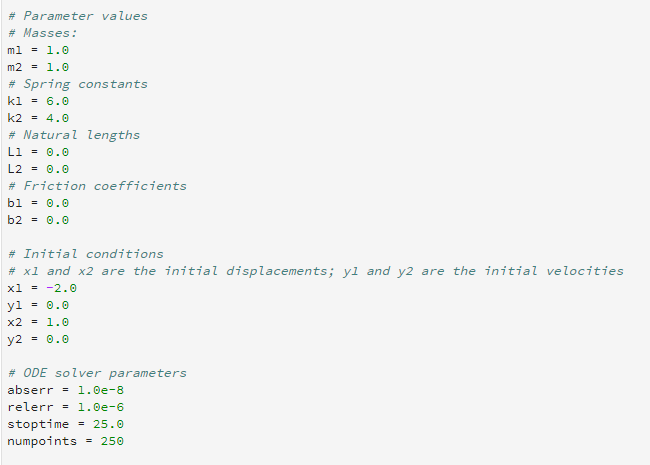
\includegraphics[width=0.65\textwidth]{Codigo2_1.PNG}
\end{figure}

Obteniendo las siguientes gráficas:
\pagebreak

\begin{figure}[ht!]
\begin{subfigure}{0.6\textwidth}
  \centering
  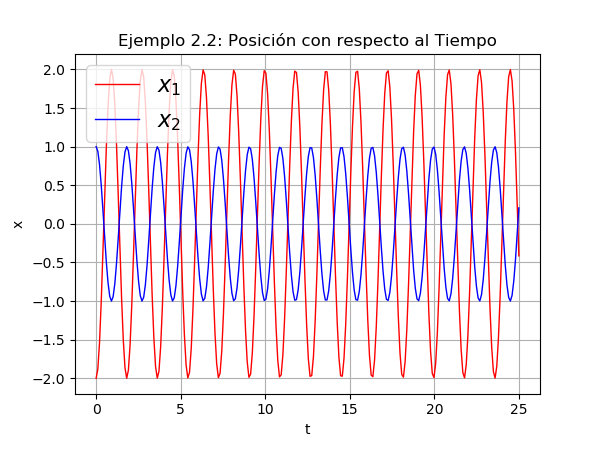
\includegraphics[width=\linewidth]{ejemplo_2_2_1.png}
   \caption{Posición con respecto al Tiempo de $x_1$ y $x_2$}
\end{subfigure}
\begin{subfigure}{0.6\textwidth}
  \centering
  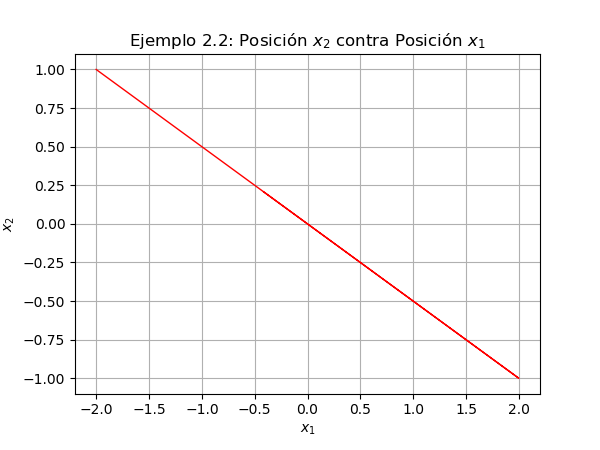
\includegraphics[width=\linewidth]{ejemplo_2_2_2.png}
  \caption{Posición $x_2$ contra $x_1$}
\end{subfigure}
\end{figure}

El error relativo de $x_1$ y $x_2$:

\begin{figure}[ht!]
\begin{subfigure}{0.6\textwidth}
  \centering
  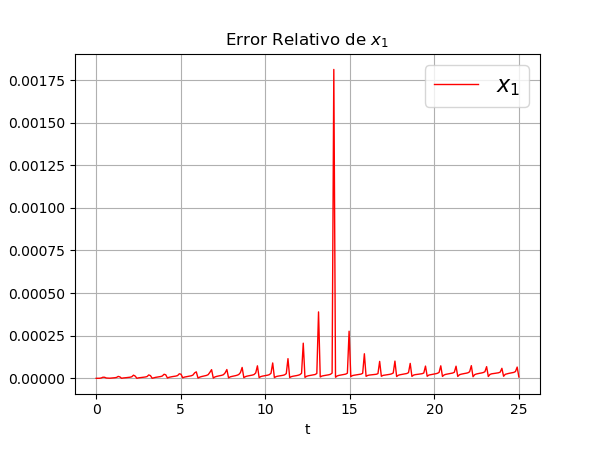
\includegraphics[width=\linewidth]{error2_2_1.png}
   \caption{Error Relativo de $x_1$}
\end{subfigure}
\begin{subfigure}{0.6\textwidth}
  \centering
  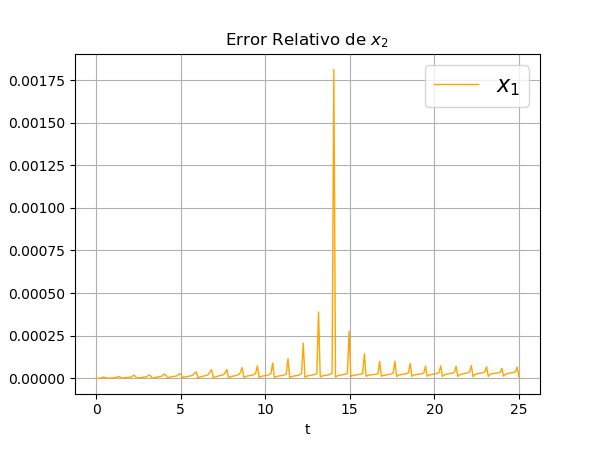
\includegraphics[width=\linewidth]{error2_2_2.png}
  \caption{Error Relativo de $x_2$}
\end{subfigure}
\end{figure}

\textbf{Ejemplo 2.3:} Describe el movimiento para las constantes de resorte $k_1 = 0.4$ y $k_2 = 1.808$ con las condiciones iniciales ($x_1(0), \dot x_1(0), x_2(0), \dot x_2(0)) = (1/2,0,-1/2,7/10)$.

En este problema, los valores de las constantes del resorte determinan el periodo y por lo tanto, la frecuencia; mientras que las condiciones iniciales solo afectan la amplitud y la fase de las soluciones. El código modificado para hacer tales gráficas resulta así:

\begin{figure}[ht!]
 \centering
  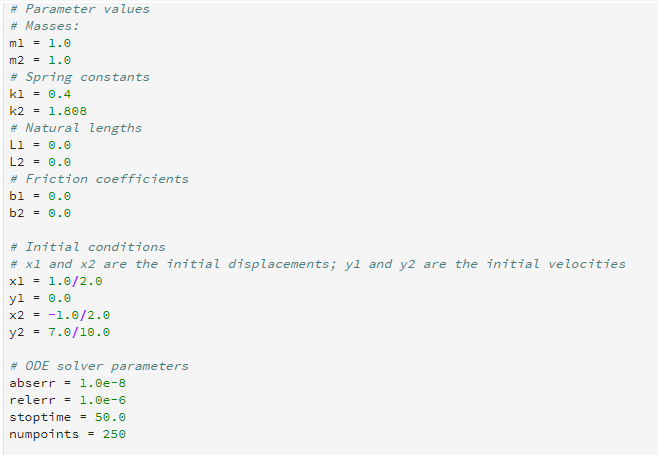
\includegraphics[width=0.65\textwidth]{Codigo2_2.PNG}
\end{figure}
 
Al graficar las soluciones, podemos ver varios patrones interesantes:

\begin{figure}[ht!]
\begin{subfigure}{0.6\textwidth}
  \centering
  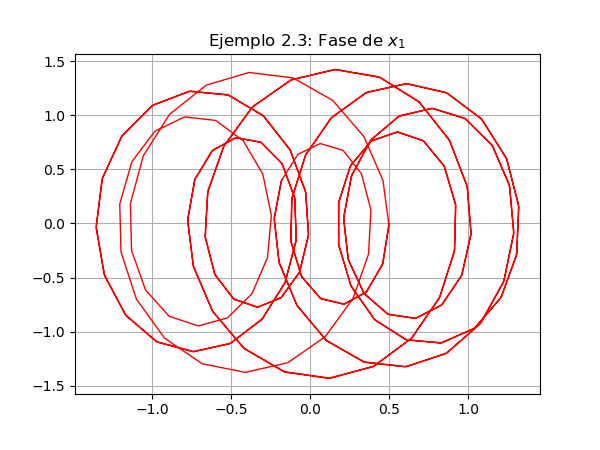
\includegraphics[width=\linewidth]{ejemplo_2_3_5.png}
   \caption{Fase para $x_1$}
\end{subfigure}
\begin{subfigure}{0.6\textwidth}
  \centering
  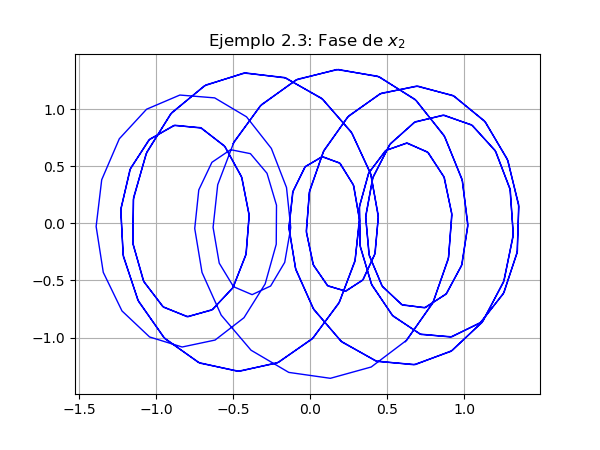
\includegraphics[width=\linewidth]{ejemplo_2_3_6.png}
  \caption{Fase para $x_2$}
\end{subfigure}
\begin{subfigure}{0.6\textwidth}
  \centering
  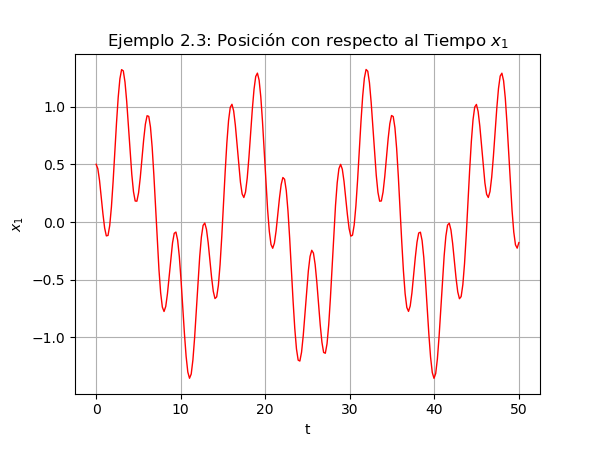
\includegraphics[width=\linewidth]{ejemplo_2_3_2.png}
  \caption{Posición con respecto al tiempo de $x_1$}
\end{subfigure}
\begin{subfigure}{0.6\textwidth}
  \centering
  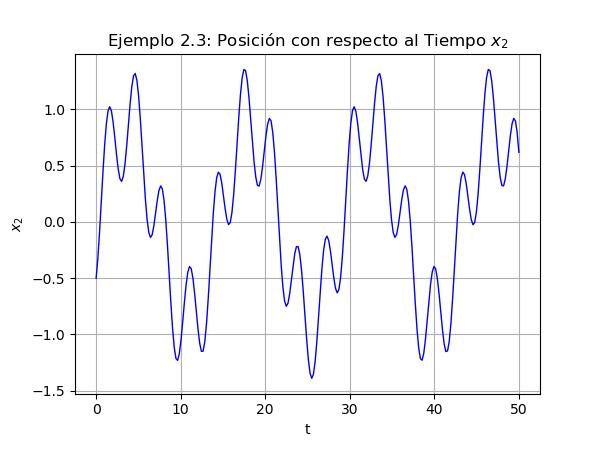
\includegraphics[width=\linewidth]{ejemplo_2_3_3.png}
  \caption{Posición con respecto al tiempo de $x_2$}
\end{subfigure}
\end{figure}
\begin{figure}[ht!]
\begin{subfigure}{0.6\textwidth}
  \centering
  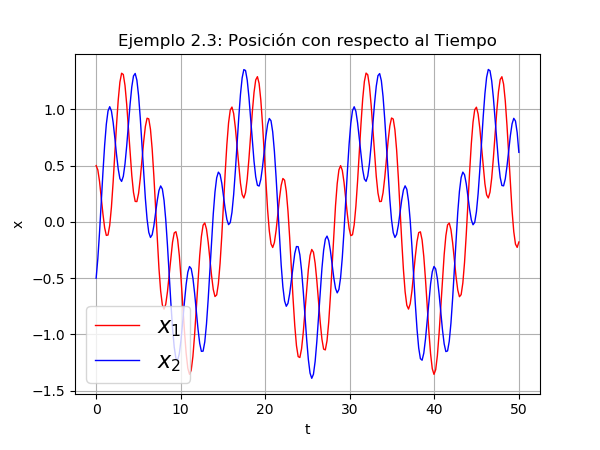
\includegraphics[width=\linewidth]{ejemplo_2_3_1.png}
  \caption{Posición con respecto al tiempo de $x_1$ y $x_2$}
\end{subfigure}
\begin{subfigure}{0.6\textwidth}
  \centering
  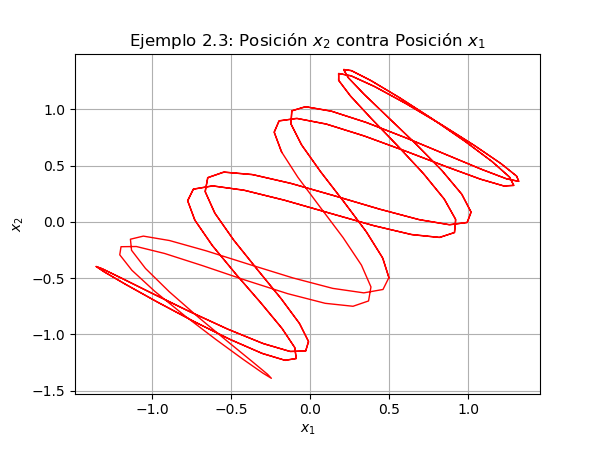
\includegraphics[width=\linewidth]{ejemplo_2_3_4.png}
  \caption{Posición $x_2$ contra $x_1$}
\end{subfigure}
\end{figure}

\subsubsection{Amortiguamiento}
El tipo de amortiguamiento más común, son los de viscosidad, donde la fuerza amortiguadora es proporcional a la velocidad. El amortiguamiento de la primera masa depende solamente de su velocidad y no de la velocidad de la segunda masa y vice versa. Para modelar esto, agregamos los términos $-\delta_1\dot x_1$ a la primera ecuación y $-\delta_1\dot x_2$ a la segunda. Asumiendo que los coeficientes de amortiguamiento $\delta_1$ y $\delta_2$ son pequeños, el modelo se da por:

\begin{center}
$m_1\ddot x_1 = - \delta_1\dot x_1 - k_1x_1 - k_2(x_1 - x_2)$

$m_2 \ddot x_2 = - \delta\dot x_2 - k_2(x_2 - x_1)$
\end{center}

Ahora, para hacer una ecuación que solo dependa de $x_2$, podemos resolver la segunda ecuación para $x_1$ y sustituirlo en la primera, obteniendo una ecuación de cuarto orden:

\begin{center}
$m_1m_2x_2^{(4)} + (m_1\delta_1 + m_2\delta_2)\dddot x_2 + (m_2k_1 + k_2(m_1 + m_2) + \delta_1\delta_2)\ddot x_2 + (k_1\delta_2 + k_2(\delta_1 + \delta_2)\dot x_2 + k_1k_2x_2 = 0$

Podemos hacer el mismo procedimiento para que dependa de $x_1$. Con esto, obtenemos una ecuación diferencial lineal que representa el movimiento de ambas pesas. 

\textbf{Ejemplo 2.4:} Asuma que $m_1 = m_2 = 1$. Describe el movimiento para las constantes de resorte $k_1 = 0.4$ y $k_2 = 1.808$, los coeficientes de amortiguamiento $\delta_1 = 0.1$ y $\delta_2 = 0.2$ con las condiciones iniciales ($x_1(0), \dot x_1(0), x_2(0), \dot x_2(0)) = (1,1/2,2,1/2)$.

Se puede observar un patrón regular en donde el movimiento avanza con una disminución en su amplitud. El código para graficar las soluciones resulta así:

\begin{figure}[ht!]
 \centering
  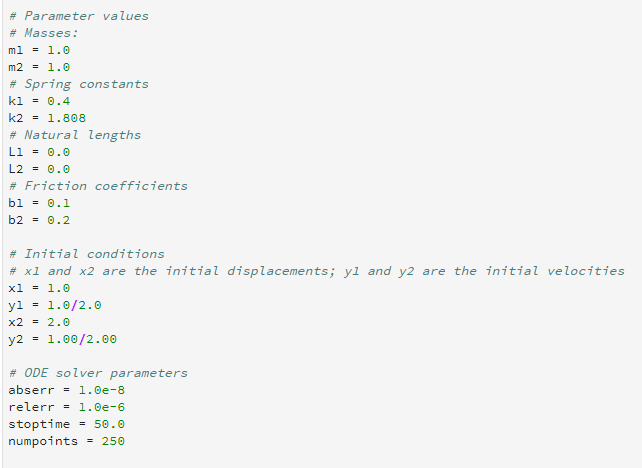
\includegraphics[width=0.65\textwidth]{Codigo2_3.PNG}
\end{figure}
 
\pagebreak

\raggedright Resultando en las siguientes graficas

\begin{figure}[ht!]
\begin{subfigure}{0.6\textwidth}
  \centering
  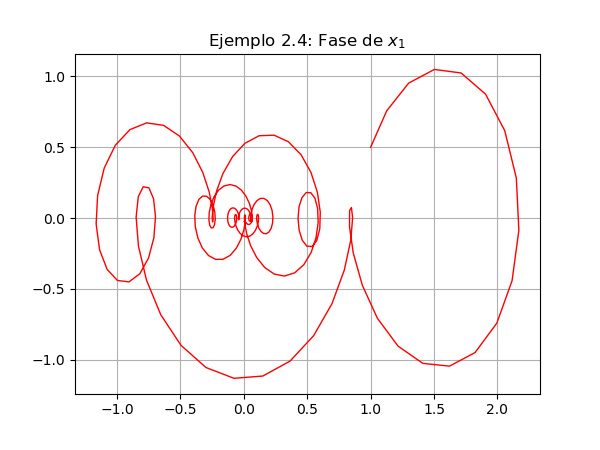
\includegraphics[width=\linewidth]{ejemplo_2_4_5.png}
   \caption{Fase para $x_1$}
\end{subfigure}
\begin{subfigure}{0.6\textwidth}
  \centering
  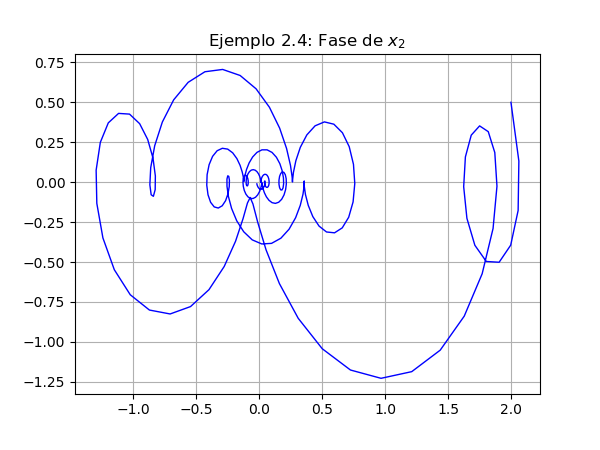
\includegraphics[width=\linewidth]{ejemplo_2_4_6.png}
  \caption{Fase para $x_2$}
\end{subfigure}
\begin{subfigure}{0.6\textwidth}
  \centering
  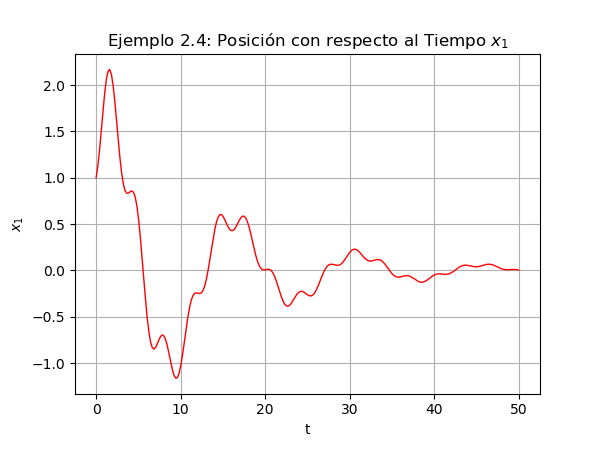
\includegraphics[width=\linewidth]{ejemplo_2_4_2.png}
  \caption{Posición con respecto al tiempo de $x_1$}
\end{subfigure}
\begin{subfigure}{0.6\textwidth}
  \centering
  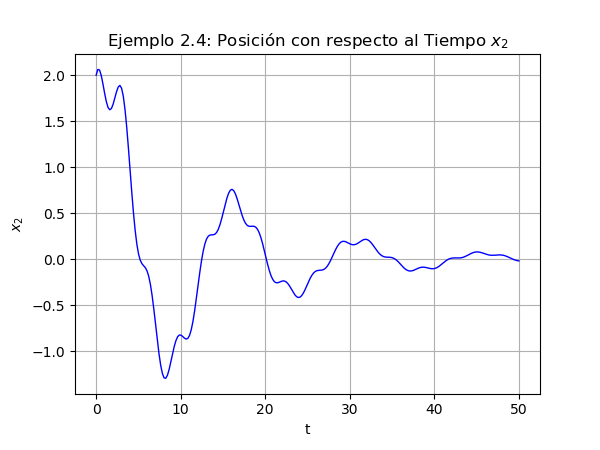
\includegraphics[width=\linewidth]{ejemplo_2_4_3.png}
  \caption{Posición con respecto al tiempo de $x_2$}
\end{subfigure}
\begin{subfigure}{0.6\textwidth}
  \centering
  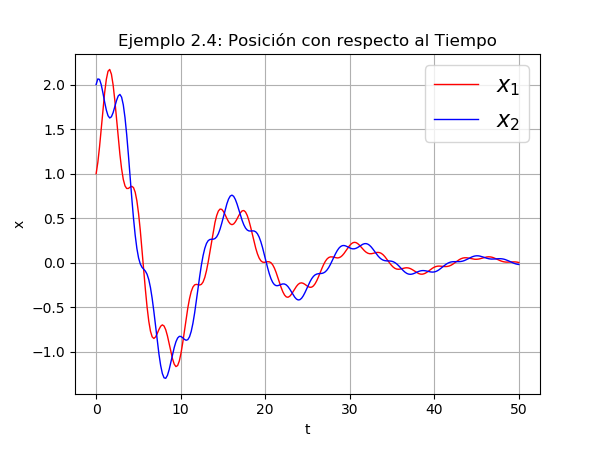
\includegraphics[width=\linewidth]{ejemplo_2_4_1.png}
  \caption{Posición con respecto al tiempo de $x_1$ y $x_2$}
\end{subfigure}
\begin{subfigure}{0.6\textwidth}
  \centering
  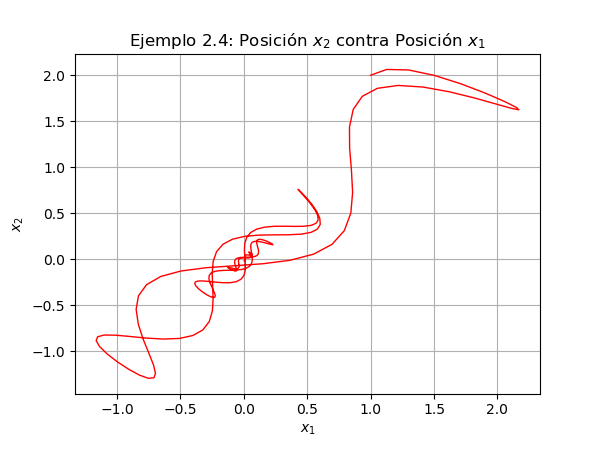
\includegraphics[width=\linewidth]{ejemplo_2_4_4.png}
  \caption{Posición $x_2$ contra $x_1$}
\end{subfigure}
\end{figure}

\section{Conclusión}

Ha sido muy interesante trabajar con esta actividad, porque es la primera vez utilizando ecuaciones diferenciales en la programación, aunque el código ya estaba hecho, el ver como trabaja y entender como funciona fue algo nuevo. Ademas de que se unieron con conceptos vistos en cursos anteriores, lo que a mi parecer, lo hizo más llamativo. Por otra parte, Jupyter Lab ha sido de más agrado que Jupyter Notebook, por cosas como la interfase, hasta el explorador de archivos que incluye a la izquierda, lo hizo más agradable y fácil de utilizar. En pocas palabras, la actividad ha sido realizada con éxito y sin mucha dificultad, y se espera poder continuar trabajando con esta seguridad y constancia en las futuras actividades del curso. 

\section{Bibliografía}
\begin{enumerate}
\item Fay, T., Graham, S. (2003) Coupled Srping Equations. Recuperado el 17 de Marzo del 2018 desde http://math.oregonstate.edu/~gibsonn/Teaching/MTH323\-010S15/Supplements/coupled\_spring.pdf

\end{enumerate}

\section{Apéndice}
\begin{enumerate}
\item \textbf{¿En general te pareció interesante esta actividad de modelación matemática? ¿Qué te gustó mas? ¿Qué no te gustó?}

La actividad me pareció muy interesante, fue muy entretenido ver como pequeños cambios iban afectando las gráficas. Lo único que no me gustó fue que el código ya estaba totalmente hecho, hubiera estado más interesante si hubiera sido más como una plantilla y no que ya estuviera totalmente desarrollado. 

\item \textbf{La cantidad de material te pareció ¿bien?, ¿suficiente?, ¿demasiado?}

Sí, estuvo muy bien y fácil de entender, ya que eran conceptos previamente estudiados en el curso de mecánica 2, aplicados en la programación.

\item \textbf{¿Cuál es tu primera impresión de Jupyter Lab?} 

Parece una versión más avanzada de Jupyter Notebook, además de que tener los archivos a la mano en la sección de la izquierda, hace todo más fácil, por lo que fue muy agradable trabajar con esta herramienta.

\item \textbf{Respecto al uso de funciones de SciPy, ¿ya habías visto integración numérica en tus cursos anteriores? ¿Cuál es tu experiencia?}

Habíamos visto integración numérica antes en otros cursos que incluían programación en FORTRAN, pero nunca con Python.

\item \textbf{El tema de sistema de masas acopladas con resortes, ¿ya lo habías resuelto en tu curso de Mecánica 2?}  

Sí, pero con mucha ayuda del profesor y sin entender muy bien que sucedía, pues aún no veíamos los temas necesarios en el curso de Ecuaciones Diferenciales. 

\item \textbf{¿Qué le quitarías o agregarías a esta actividad para hacerla más interesante y divertida?}

La práctica tal y como esta estuvo bien, no fue ni muy tediosa, ni complicado, pero tampoco muy fácil. En pocas palabras, fue una actividad muy amena. 
\end{enumerate}

\end{center}

\end{document}